\documentclass[twocolumn,a4paper]{article}
\usepackage[top=1cm, bottom=2.5cm, left=2.5cm, right=2.5cm]{geometry}
\usepackage{graphicx} % Required for inserting images
\usepackage{hyperref} % Required for \url command
\usepackage{xcolor}
\usepackage{everypage}

\AddEverypageHook{%
  \begin{picture}(0,0)
    \put(-42,-420){\rotatebox{90}{\color{gray!60}\fontsize{28}{32}\selectfont\textsc{Checkpoint Report}}}
  \end{picture}%
}

\title{Simulation of a computer game by diffusion model\footnote{\url{https://github.com/MichaelPestuka/KNN_proj}}}
\author{
  Lukáš Foukal \and
  David Nepraš \and
  Michael Peštuka
}
\date{April 2026}

\begin{document}

\maketitle

\section{Problem}
The goal of our project is to create a playable simulation of a computer game by using a diffusion model. For such a model, the input is the previous frame (or a sequence of frames) and the user action. The output is the next frame. Various computer games have already been simulated using this approach.

\section{Data generation}

For generating the training data, a Mario Brothers emulator \footnote{\url{https://github.com/Kautenja/gym-super-mario-bros}} was used, as the Gymnasium framework did not have the NES game we were looking for. For controlling the game while generating the data, three strategies were originally used. The first was fully random, with a uniform distribution of all the provided \texttt{SIMPLE\_MOVEMENT} actions and some action stickiness over several frames. The second strategy relied on a pre-trained AI\footnote{\url{https://github.com/yumouwei/super-mario-bros-reinforcement-learning}}, and the third was a combination with random-length few-second periods of one or the other.

This combination led to very good coverage of the first level of the game; see figure \ref{fig:level_coverage}.

\begin{figure*}
  \centering
  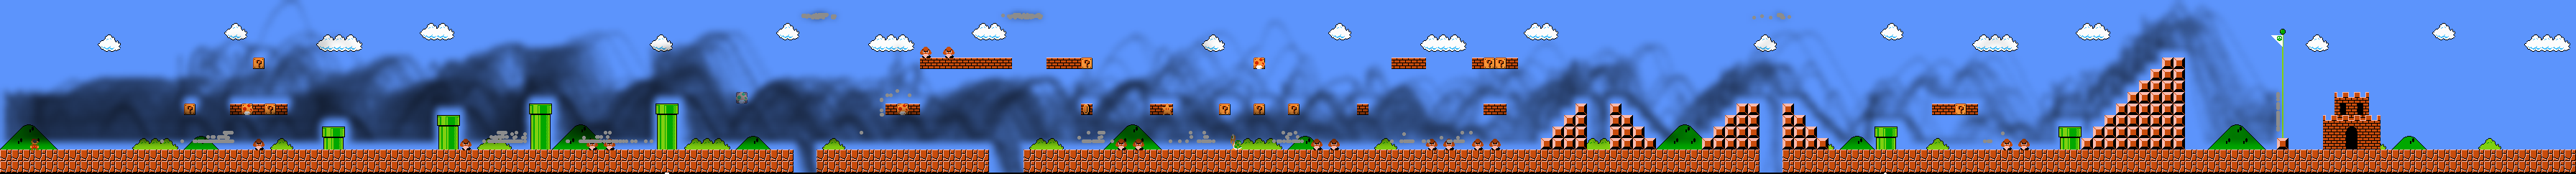
\includegraphics[width=\textwidth]{figures/mario_w1s1_original_dataset_heatmap_overlay_1101runs.png}
  \caption{A map of level coverage}
  \label{fig:level_coverage}
\end{figure*}

The character trajectories were also very varied, see \ref{fig:level_trajectories}.

% ONE OF THESE TWO FIGURES CAN PROBABLY GO. WHICH DO YOU LIKE BETTER? 

\begin{figure*}
  \centering
  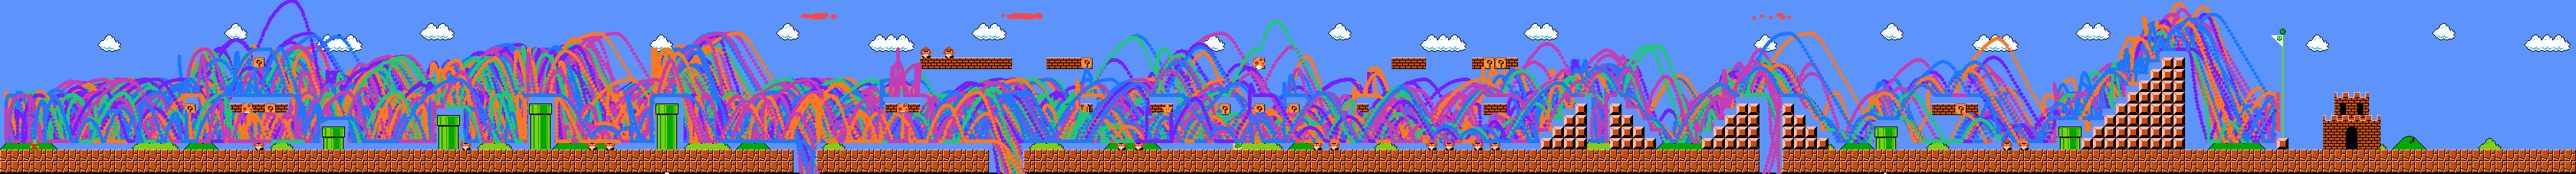
\includegraphics[width=\textwidth]{figures/mario_w1s1_original_dataset_dots_overlay_1101runs.png}
  \caption{A map of level trajectories}
  \label{fig:level_trajectories}
\end{figure*}

The first attempt training mix (seen in these figures) was 1000 runs of combined, 100 of fully random and only one run off the optimal AI policy, given that was pixel perfect repeatable. This did not turn out to be and optimal mix, along with another issue not entirely visible from the validation images shown here.

The \texttt{SIMPLE\_MOVEMENT} control mechanism provided by the emulator does allow for movement \texttt{left} and \texttt{right}, but only has combinations with the \texttt{A} and \texttt{B} keys for the \texttt{right}, so 4 of the possible 7 actions move the game character forward. This was also exacerbated by the AI strategy, which used these actions even more than the uniform random distribution. This resulted in our original training dataset of 665 816 images only containing 5,42\% \texttt{left} actions. As a consequence of these imbalances, our first round of models continued moving the character forward even without user input.

In our enhanced dataset, this was increased to 17,05\% while also increasing the number of frames where no action was taken from 14,81\% to 50,05\%. The impact of this change on our second generation of model checkpoints is not yet known.

\section{GameNGen architecture}
\label{gamengen}

GameNGen\footnote{\url{https://arxiv.org/abs/2408.14837}} is an architecture originally developed for simulating the video game DOOM. It is based on a pre-trained text-to-image model, speciffically Stable Diffusion 1.4. This model is used to predict the next frame given the sequence of previous actions (player inputs) and observations (frames). Each action from the sequence is encoded into a single token, which are then used to replace the cross attention from text encoding generally used by Stable Diffusion. The sequence of frames is encoded using the autoencoder and then concatenated to the noised latents in the latent channels dimension.

Since the code for the official GameNGen implementation is not public, we are currently experimenting with an unofficial reproduction\footnote{\url{https://github.com/arnaudstiegler/gameNgen-repro}}. This implementation has reached similar results in regards to visual quality, however it doesn't reach 20 FPS as reported in the original paper.

\subsection{Preventing autoregressive drift}
Generating frames autoregressively can lead to error accumulation and eventual incoherence. To combat this, context frames are 'corrupted' during training by adding a varying level of gaussian noise, while providing the noise level as an input to the model. During inference the added noise level can be controlled for maximal quality.

\subsection{Autoencoder finetuning}
The authors of GameNGen have found that using the pretrained autoencoder provided by Stable Diffusion results in meaningful artefacts and blurry UI elements. This is also consistent with our own findings. To mitigate this, only the decoder is finetuned to preserve the pre-trained knowledge of the diffusion model. This process is completely separate from the U-Net training and also doesn't affect autoregressive generation, since it uses only the latents and not pixels.

\subsection{Current status}

Video sequences generated by this method are visually impressive, reaching similar visual quality to the original data. However we are currently experiencing the fact, that when trying to use the model interactively, the player controls are far from responsive. For example the model tries to move right in most situations, even when no buttons are pressed. We suspect that this is due to movement to the right being overrepresented in the training data.


\section{ControlNet based approach}
\label{controlnet}

In this section, we review the foundational literature and prior research that inspire this specific component of our project. We focus primarily on the advancements in conditional image generation through diffusion models, most notably ControlNet, and outline the conceptual framework that guided our implementation. By contextualizing these generative technologies alongside the principles of sequential world modeling, we highlight the rationale behind our specific approach: decoupling the underlying game logic and state prediction from the final visual rendering process.

% @PRASA I AM GONNA NEED SOME ROLLOUTS AND THEIR GROUND TRUTH DATA FOLDERS TO INCLUDE THE MODEL IN EVALUATION SECTION, OR A GUIDE ON HOW TO RUN IT. HAVE NOT TRIED YET, MAYBE THE LLMS CAN FIGURE IT OUT

% \subsection{Related work and inspiration}

\subsection{Conditional Image Generation via ControlNet}

While traditional diffusion models have achieved remarkable success in high-fidelity image generation, controlling their exact spatial layout using text prompts alone remains highly challenging. To address this limitation, Zhang et al. (2023) introduced ControlNet\footnote{\url{https://arxiv.org/abs/2302.05543}}, an architecture designed to add spatial conditioning controls to large, pre-trained text-to-image diffusion models. By locking the original model weights and training a parallel "copy" of the encoding layers, ControlNet enables the injection of explicit structural priors—such as semantic segmentation masks, depth maps, or Canny edges—without destroying the base model's prior knowledge.  This capability to deterministically guide the structural composition of the output is foundational to our approach, as it provides a robust mechanism to translate abstract, low-dimensional game states (represented as segmentation maps) into two-dimensional game-like visual frames.

\subsection{Extensions for Video Generation}

Although ControlNet excels at conditional static image generation, applying it naively on a frame-by-frame basis for game simulation inherently leads to temporal inconsistency, often manifested as severe visual flickering or morphological shifting. To mitigate this within the diffusion process itself, subsequent research introduced temporal extensions such as ControlVideo\footnote{\url{https://arxiv.org/abs/2305.13077}}. These methods typically incorporate cross-frame attention mechanisms and temporal smoothing directly into the diffusion pipeline to ensure coherence across sequences. However, our project specifically diverges from this approach; we do not utilize these native video-diffusion extensions. Instead, we isolate the problem of temporal consistency by handling the sequential dynamics entirely outside the diffusion rendering phase.

\subsection{World Models and Sequential Game Simulation}

The concept of learning the internal dynamics of an environment to simulate future states was popularized by Ha and Schmidhuber (2018)\footnote{\url{https://arxiv.org/abs/1803.10122}} through the paradigm of World Models. In their foundational work, an agent learns a compressed spatial representation of a game environment and utilizes a sequence model to predict future latent states based on current observations and player actions. Our architecture integrates this philosophy into the diffusion-based pipeline. Rather than relying on a video diffusion model to guess temporal changes, we employ a Transformer architecture to act as our predictive World Model. The Transformer is explicitly responsible for computing the temporal physics, game logic, and state transitions, ultimately outputting a predicted structural layout for the next frame. Consequently, the ControlNet acts purely as a conditioned rendering engine. This decoupling of "game logic" (handled by the Transformer) and "graphics rendering" (handled by ControlNet) creates a highly controllable and cohesive game simulation pipeline.

\subsection{Architectural Design and Inference Pipeline}

Our implementation explicitly decouples state prediction from visual rendering to maximize control and stability. The core predictive engine is a Transformer-based world model that processes sequential concatenations of physical coordinates, player actions, and compressed visual latents (extracted via a frozen Autoencoder and a custom CNN compressor). Instead of directly outputting RGB pixels, the Transformer predicts a latent representation of the next state, which is subsequently upsampled by a custom decoder into a multi-class semantic segmentation mask. This intermediate mask serves as the explicit structural bridge to the generative phase. For rendering, we utilize a pre-trained Stable Diffusion model coupled with a semantic ControlNet. The ControlNet simply receives the upscaled segmentation map as a conditioning image, deterministically guiding the diffusion pipeline to render high-fidelity frames that obey the Transformer's underlying spatial and physical logic.

\subsection{Progressive Training Schema and Tailored Objectives}

To mitigate the autoregressive drift—a critical challenge in long-horizon game simulation—we employ a phased, multi-step rollout training curriculum. The Transformer and decoder are trained end-to-end, beginning with single-step teacher forcing and progressively scaling up to 100-step autoregressive sequences to force the model to recover from its own accumulated errors. Furthermore, the architecture is optimized using a highly specialized composite loss function to handle the unique domain of 2D game rendering. Alongside standard Binary Cross-Entropy, we integrate a soft Dice loss to heavily penalize errors on small, sparse objects (such as the player or enemies) and a boundary loss (utilizing Sobel edge detection) to enforce crisp semantic borders. Most notably, we introduce a physics-gated spatial loss: by applying a Gaussian prior centered around the Transformer's predicted physical coordinates, the loss function explicitly restricts where the player character can be visually generated, ensuring strict consistency between the internal game physics and the final visual output.
\section{Interactive}

Given our reliance on high-power cloud infrastructure for training and inference, we have created a client-server type application for trying out the model interactively, like a real game. Because this is just for testing purposes, it is in the form of a portable Python GUI application which initiates an SSH session with our remote VPS, starts the inference process there, and then streams JPEG-encoded images back while user actions are streamed to the server.

For this inference mode on the GameNGen architecture model, only 3 diffusion steps are used. We have also employed a handful of optimizations beyond the latent image buffer used in the base model (see \ref{gamengen}). One of these optimizations is using 16-bit floating-point values instead of the original 32-bit. Even though a latent buffer is used and only the output image needs to be run through the VAE for display, this task was offloaded to a second GPU along with encoding the image into JPEG for transport, keeping the primary GPU running the UNet continuously. This increased FPS by about 12\%. As of the writing of this report, we are achieving around 22,5 FPS on a pair of Nvidia RTX PRO 6000 Blackwell GPUs while only utilizing them to about 50\% and 10\% respectively. This results in the relatively tame power draw of only 300W combined, about half of the TDP of one of these GPUs.

Currently we do not have a remote interactive application of the ControlNet based model.

\section{Evaluation}

While we discussed PSNR previously, we are currently focusing on less pixel-level, more perceptual metrics. One of these is LPIPS (Learned Perceptual Image Patch Similarity) \footnote{\url{https://arxiv.org/abs/1801.03924}}, which is also cited in the GameNGen paper. This metric is also available from a PyPI package from the authors of the paper\footnote{\url{https://pypi.org/project/lpips/\#1-learned-perceptual-image-patch-similarity-lpips-metric}}.

We have employed both PSNR and LPIPS in an evaluation script, but currently our models generate images outside the scope of this kind of evaluation, failing to model primary game mechanics.

% I WILL REDO THIS VALIDATION TOMORROW ON BOTH THE OG DATA 250k AND SECOND GEN GAMENGEN MODEL

\section{Future work}

Currently we are focusing on re-running our training with the updated dataset. If this section hasn't been updated with the results then something probably went wrong.

Further, I would like to explore training a smaller, purpose-built transformer from the ground up to achieve better performance on more reasonable hardware, like a laptop GPU.

I encourage my colleagues to add to this section, of course.

\end{document}
